\documentclass[11pt]{article}

% ── Encoding & fonts ──────────────────────────────────────────────────────────
\usepackage[T1]{fontenc}
\usepackage[utf8]{inputenc}
\usepackage{lmodern}
\usepackage{microtype}

% ── Page geometry ─────────────────────────────────────────────────────────────
\usepackage[margin=1.25in]{geometry}

% ── Mathematics ───────────────────────────────────────────────────────────────
\usepackage{amsmath}
\usepackage{amssymb}
\usepackage{amsthm}

% ── Tables ────────────────────────────────────────────────────────────────────
\usepackage{booktabs}
\usepackage{array}
\usepackage{tabularx}

% ── Lists ─────────────────────────────────────────────────────────────────────
\usepackage{enumitem}
\setlist{itemsep=2pt, topsep=4pt}

% ── Code / typewriter text ────────────────────────────────────────────────────
\usepackage{listings}
\lstset{basicstyle=\ttfamily\small, breaklines=true}

% ── Hyperlinks ────────────────────────────────────────────────────────────────
\usepackage[colorlinks=true, linkcolor=black, citecolor=black,
            urlcolor=black, pdfborder={0 0 0}]{hyperref}
\usepackage{url}

% ── Bibliography ──────────────────────────────────────────────────────────────
\usepackage[numbers, sort&compress]{natbib}
\bibliographystyle{unsrtnat}

% ── Paragraph spacing ─────────────────────────────────────────────────────────
\usepackage{parskip}
\setlength{\parskip}{6pt}

% ── Section formatting ────────────────────────────────────────────────────────
\usepackage{titlesec}
\titleformat{\section}{\large\bfseries}{\thesection.}{0.6em}{}
\titleformat{\subsection}{\normalsize\bfseries}{\thesubsection}{0.6em}{}
\titlespacing{\section}{0pt}{14pt}{6pt}
\titlespacing{\subsection}{0pt}{10pt}{4pt}

% ── Figures (tikz/pgfplots for the empirical section) ───────────────────────
\usepackage{tikz}
\usepackage{pgfplots}
\pgfplotsset{compat=1.18}

% ── Abstract ──────────────────────────────────────────────────────────────────
\usepackage{abstract}
\renewcommand{\abstractnamefont}{\normalfont\bfseries}
\renewcommand{\abstracttextfont}{\normalfont\small}

% ── Footnotes ─────────────────────────────────────────────────────────────────
\usepackage[hang, flushmargin]{footmisc}

% ── Theorem environments ──────────────────────────────────────────────────────
\theoremstyle{definition}
\newtheorem{definition}{Definition}

\theoremstyle{plain}
\newtheorem*{informaltheorem}{Theorem (informal)}

\theoremstyle{plain}
\newtheorem*{property}{Property}

% ─────────────────────────────────────────────────────────────────────────────
\title{\textbf{Heterogeneous Local Knowledge Systems:\\
A Formal Framework for Cross-Domain\\
Coordinator-Free Substrate Design}}

\author{%
  Dr.\ Richard Nicholson\\[4pt]
  \small Tathata Systems Ltd, United Kingdom\\
  \small \href{mailto:tathatasystems@proton.me}{tathatasystems@proton.me}
}

\date{June 2026\\[4pt]
\small Preprint. Companion to~\cite{nicholson2026}.}
% ─────────────────────────────────────────────────────────────────────────────

\begin{document}

\maketitle

\begin{abstract}
The companion paper~\cite{nicholson2026} argues that mediated multi-agent
architectures exhibit structural failure modes irreducible by engineering effort,
and derives a coordinator-free substrate from Holland's signal/boundary model. In
its Discussion, it observes that the failure modes parallel Hayek's 1945
argument against central economic planning and Beinhocker's empirical analysis
of hierarchical organisations, but qualifies the observation as ``suggestive
rather than exact---economies, biological systems, and distributed software are
not identical.'' This paper argues that the parallel is, in fact, structurally
exact, and supplies the formal framework that makes it so. We introduce
\emph{Heterogeneous Local Knowledge Systems} (HLKS) as the common abstraction
underlying four independent intellectual traditions: economic epistemics
(Hayek), polycentric commons governance (Ostrom), organisational adaptation
(Beinhocker), and distributed computing (Holland, and the companion paper). We
state the \emph{Coordinator Trap Theorem} informally and argue that for any
HLKS satisfying mild heterogeneity and state-change conditions, any coordinator
mechanism accumulates epistemic error proportional to scale and heterogeneity,
while a locally-resolved signal mechanism does not. We then identify four
substrate correctness properties that follow from the theorem and show that
they are independently derived---in different vocabularies, with different
formal apparatus, across more than half a century---in each of the four
traditions. We extend the MCB/P/S evaluative framework (Moral Circle Breadth,
Polycentricity, Surplus-Claim Regime) from monetary system design to substrate
design generally, showing that it captures the same structural distinctions
across domains. We distinguish two grades of local resolution---locally evaluated
\emph{prediction}, which shrinks the coordinator's epistemic error, and
self-resolved \emph{pull}, which eliminates the variable in which that error
is expressed: a worker that claims work when ready makes the only promise a
distributed agent can always keep, because making it and keeping it are the
same event. We anchor the framework in the computing domain in both grades:
a measurement on a single substrate in which broker-mediated decisions
exhibit mean latency two to three orders of magnitude higher than locally
evaluated ones (the within-paradigm gradient the theorem predicts), and a
constructive pull instantiation---a tuple-space layer built entirely from
the substrate's public primitives---whose test suite verifies exactly-once
distribution with no participant holding a view of any other's state, and
survival of the rendezvous point itself through emergent, coordinator-free
failover. We close with an
honest accounting of the open questions:
the formal status of the theorem, the boundary conditions of the HLKS model,
the Holland/Burgess tension, and the further structural properties that
correctness against external and internal capture would require---properties
that are the subject of a companion paper currently in preparation.
\end{abstract}

% ─────────────────────────────────────────────────────────────────────────────
\section{Introduction}

In \S9.1 of the companion paper~\cite{nicholson2026}, the coordinator trap---a
structural failure mode of mediated multi-agent architectures---is observed to
parallel Hayek's epistemic argument against central economic
planning~\cite{hayek1945}. The paper notes that ``a planned economy and a
mediated hierarchy share a recognisable failure mode: a central node that must
aggregate knowledge it cannot fully possess, synthesise decisions on behalf of
participants who understand their local context better than any coordinator
can, and issue commands downward into a system whose ground truth is always
more current at the edges than at the centre.'' \S9.2 adds Beinhocker's
empirical analysis of hierarchical organisations~\cite{beinhocker2006} as a
third independent direction arriving at the same conclusion. The paper then
qualifies: ``The parallel to the coordinator trap is suggestive rather than
exact---economies, biological systems, and distributed software are not
identical.''

This paper argues that the parallel is, in fact, structurally exact. The
qualification in~\cite{nicholson2026} is correct as an honest statement of
what that paper had established---a single-domain architectural argument with
two cross-domain observations in its Discussion---but understates what is
available with the right abstraction. With an appropriate formal model of
the underlying problem, the four traditions can be shown to be solving
\emph{the same problem}, not merely \emph{analogous problems}; their
prescriptions converge because the structure of the problem admits only one
class of correct solution.

The contributions of this paper are:

\begin{enumerate}
\item A formal abstraction---the \emph{Heterogeneous Local Knowledge System}
  (HLKS)---common to economic, governance, organisational, and computing
  domains, expressed as a five-component tuple capturing the agents, their
  heterogeneous local knowledge, the rate at which that knowledge changes, the
  communication latency between agents, and the optimal decision function the
  system is attempting to approximate.

\item An informal statement of the \emph{Coordinator Trap Theorem}, with a
  careful argument that for any HLKS satisfying mild heterogeneity and
  state-change conditions, any coordinator-based mechanism accumulates
  epistemic error that grows with scale, heterogeneity, and the rate of
  state change, while a locally-resolved signal mechanism does not.

\item Four independent domain instantiations of the HLKS framework, together
  with a structural identity table that makes the cross-domain correspondence
  precise rather than analogical.

\item Generalisation of the MCB/P/S evaluative framework (Moral Circle
  Breadth, Polycentricity, Surplus-Claim Regime), originally developed for
  monetary system design, to substrate design generally---and a demonstration
  that the three axes capture exactly the structural distinctions the
  Coordinator Trap Theorem implies a correct substrate must exhibit.

\item Statement of four substrate correctness properties that follow from
  the framework and appear in each of the four traditions: local signal
  propagation, emergent group formation, minimal federation invariants, and
  subsidiarity-respecting consensus.

\item A single-domain empirical anchoring in two parts: a measurement in
  which the same Mycelium substrate is configured into either prediction
  pattern (broker-mediated or locally evaluated) via $\sim$20 lines of
  mode-specific code and the decision-latency gap predicted by the
  framework is measured directly; and a constructive pull
  instantiation---a tuple-space companion layer built entirely from the
  substrate's public primitives---whose behavioural test suite verifies
  the framework's strongest claim, that self-resolved action eliminates
  rather than reduces the coordinator's epistemic error term.

\item An honest accounting of the open questions: the formal status of the
  theorem, the HLKS boundary conditions, the Holland/Burgess tension on
  emergent higher-order structures, and the further properties that
  correctness against political capture would require (subject of a
  companion paper).
\end{enumerate}

The implication of the framework is not that coordinator-based architectures
are universally wrong---there are domains, notably those with homogeneous
agents and low state-change rates, where the HLKS assumptions fail and
traditional consensus is well-suited. The implication is that for any system
satisfying the HLKS assumptions, the coordinator-free substrate is the
structurally correct architecture, and the convergent prescriptions of the
four traditions are evidence supporting this claim rather than independent
coincidences.

% ─────────────────────────────────────────────────────────────────────────────
\section{Heterogeneous Local Knowledge Systems}
\label{sec:hlks}

We require a formal abstraction general enough to apply across all four
domains while specific enough to support non-trivial claims. The key empirical
observation, common to economics, governance, organisations, and computing, is
that in each domain (a)~there are autonomous agents with local knowledge
states; (b)~those states are heterogeneous across agents in both structure and
content, and evolve over time; (c)~coordination is required for system-level
outcomes, but the information needed for correct coordination is distributed
across agents and not directly accessible to any single point.

\subsection{Definition}

\begin{definition}[Heterogeneous Local Knowledge System]
A \emph{Heterogeneous Local Knowledge System} (HLKS) is a tuple
$(A, K, \delta, \lambda, D)$ where:
\begin{itemize}
\item $A = \{a_1, \ldots, a_n\}$ is a finite set of autonomous agents.
\item $K = \{K_i : T \to S_i\}_{i \in A}$ is a family of local knowledge
  functions, one per agent, each mapping time $T$ to a local state space
  $S_i$. The state spaces are \emph{heterogeneous}: $S_i$ and $S_j$ are
  generally distinct in both structure and content---agents hold qualitatively
  different knowledge, not merely different values of the same variables.
\item $\delta = \{\delta_i\}_{i \in A}$ is the family of state-change rates,
  one per agent, characterising how quickly $K_i(t)$ evolves. In heterogeneous
  fleets, $\delta_i$ varies across agents.
\item $\lambda = \{\lambda_{ij}\}_{i,j \in A \cup \{C\}}$ is the family of
  communication latencies---the minimum time for information held by agent
  $i$ to become observable by agent $j$ (or by a coordinator $C$, if one is
  present).
\item $D : \prod_i S_i \to \mathit{Actions}$ is the \emph{optimal decision
  function}: the mapping from the aggregate current state of all agents to
  the action that best serves the system's objectives. $D$ requires
  \emph{current} state; stale inputs degrade output.
\end{itemize}
\end{definition}

The definition is deliberately spare. We do not specify the structure of the
state spaces beyond their heterogeneity, the precise form of $D$ beyond its
dependence on aggregate current state, or the topology of the communication
network beyond the existence of pairwise latencies. The claim is that this
minimal structure suffices to derive the Coordinator Trap, and that it
correctly characterises the common structure across the four target domains.

\subsection{The Coordinator's Epistemic Problem}

A coordinator $C$ attempting to compute $D(t)$ from a position outside the
agent population can only observe estimates $\hat{K}_i(t) = K_i(t - \lambda_{iC})$:
that is, the state of agent $i$ as it was at the moment its information was
emitted toward the coordinator, not the state at time $t$. The coordinator's
estimate of the true aggregate state is therefore always stale by at least
$\lambda_{iC}$ for each contributing agent. Critically, this is not a hardware
limitation that can be engineered away. It is a consequence of the finite
speed of information propagation, which holds under any physical
implementation regardless of available compute.

\subsection{The Coordinator Trap Theorem}

\begin{informaltheorem}[The Coordinator Trap]\label{thm:coordtrap}
For any HLKS where
\begin{enumerate}[label=(\roman*)]
\item local states are heterogeneous across agents (the state spaces $S_i$
  and $S_j$ are not isomorphic, and the values $K_i(t)$ and $K_j(t)$ are not
  derivable from one another),
\item state-change rates $\delta_i$ are bounded away from zero, and
\item the optimal decision function $D$ requires current aggregate state,
\end{enumerate}
the following hold:
\begin{enumerate}
\item The coordinator's per-agent epistemic error
  $\varepsilon_i(t) = \mathrm{dist}(K_i(t), \hat{K}_i(t))$ is strictly positive
  for all $t$ and all $i$, where $\mathrm{dist}$ is any appropriate distance
  metric on $S_i$.
\item The expected aggregate error $\mathbb{E}\!\left[\sum_i \varepsilon_i(t)\right]$
  grows monotonically with the number of agents $n$, with a measure $H$ of
  the heterogeneity of the state spaces, and with the mean state-change rate
  $\bar{\delta}$.
\item No increase in coordinator computational capacity can reduce
  $\varepsilon_i$ below the bound imposed by $\lambda_{iC}$. The constraint
  is epistemic, not computational: faster computers do not help.
\end{enumerate}
\end{informaltheorem}

\subsection{On the Formal Status of the Theorem}
\label{sec:formalstatus}

We state Theorem~\ref{thm:coordtrap} informally and argue carefully. A formal
proof would require commitment to: a specific model of the communication
medium and its latency distribution; a specific metric on local state spaces;
a specific characterisation of ``heterogeneity'' that admits a quantitative
measure $H$; and a specific decision criterion under which the optimal
function $D$ degrades with stale inputs. Each commitment is sensible for any
single domain but defeats the cross-domain generality we are attempting to
establish. In economics, the natural state metric is preference-revealed
willingness to pay; in governance, it is institutional fit; in distributed
computing, it is bytewise distance in a serialised state space. A theorem
proved in one of these formalisms does not transfer to the others.

We therefore choose to argue the theorem informally with sufficient care that
the cross-domain claim is supported, and to leave formal proof in each
specific domain to the relevant domain literature. The economics literature
contains a formal proof of part (3) for market economies under the
calculation-debate framing (Mises, Hayek, and later Hurwicz, Marschak, and
Radner on the cost of communicating decentralised information). The
distributed-systems literature contains formal lower bounds related to
part (3) in the form of impossibility results for consensus under
asynchronous network conditions (FLP). The governance and organisational
literatures argue part (3) empirically rather than formally. The contribution
of the present paper is not to prove the theorem in any single domain---each
domain has its own formal apparatus, several of them more developed than
ours---but to show that the underlying structural claim is the same across
domains, and that the convergent prescriptions of the four traditions follow
from it.

\subsection{The Locally-Resolved Alternative: Two Grades of Locality}
\label{sec:twogrades}

If the coordinator cannot compute $D(t)$ correctly, the natural question is
whether any mechanism can. We claim that a locally-resolved signal mechanism
avoids the coordinator's epistemic error by construction. Rather than
aggregating state at a central point and computing $D$ globally, each agent
applies a local filter to the signals it receives and takes an action based on
its own current state $K_i(t)$. No agent needs to know the global state; each
needs only its own state and the signals propagating through its local
neighbourhood.

It is essential---and an earlier draft of this paper failed to make the
distinction---to separate two grades of local resolution that this
description admits:

\begin{enumerate}
\item \textbf{Locally evaluated prediction.} The decision is computed at the
  edge rather than at a centre, but its \emph{inputs} are still other
  agents' states as locally observed: agent $j$ selects a target agent $i$
  by evaluating $\hat{K}_i(t) = K_i(t - \lambda_{ij})$. This removes the
  coordinator's serialisation and one propagation hop, so the error
  coefficient shrinks---but the error term has the same structure as the
  coordinator's. The decision still \emph{predicts} another agent's current
  state from a stale observation, and the prediction degrades with
  $\bar{\delta}$ exactly as Theorem~\ref{thm:coordtrap}(2) prescribes.
  Decentralising the predictor does not change what is being predicted.
\item \textbf{Self-resolved action (pull).} The allocation question is
  inverted so that every decision references \emph{only the deciding agent's
  own state}. A worker does not get selected on a prediction of its
  readiness; it \emph{announces} readiness by the act of claiming work when
  ready. The only state input is $K_i(t)$ read by agent $i$ itself, for
  which $\lambda_{ii} = 0$ and hence $\varepsilon_i \equiv 0$ identically.
  The staleness term does not become small; it becomes undefined, because
  no agent ever predicts another's state.
\end{enumerate}

The cost of locality is precision: a locally-resolved mechanism cannot
guarantee that the action taken is globally optimal in the sense $D$ would
prescribe if it had access to current aggregate state. The gain is correctness
at scale: the action each agent takes is based on information that is current
and accurate, not stale. For heterogeneous systems where the globally optimal
decision is structurally unknowable in finite latency, the locally-resolved
mechanism is not a compromise---it is the only mechanism that operates on true
information about the aggregate state. And of its two grades, only the second
realises the claim fully: grade (1) reduces the epistemic error; grade (2)
eliminates the variable in which the error is expressed.

This is the key inversion. Coordinator-based mechanisms optimise against a
specification ($D$) that they cannot evaluate correctly. Locally-resolved
mechanisms satisfy a weaker specification ($D$ on local state) that they can
evaluate exactly. Under the HLKS conditions, the second is the strongest
specification that any architecture can correctly satisfy---and the pull
grade is its exact realisation, not an approximation of it.

\subsection{The Promise-Theoretic Reading: Assessments Mistaken for Promises}
\label{sec:promisereading}

Burgess's Promise Theory~\cite{burgess2018,burgess2013} supplies the precise
vocabulary for \emph{why} the prediction paradigm fails, in any grade. In
Promise Theory an agent can make promises only about its own behaviour;
statements about another agent are \emph{assessments}, local and ephemeral.
A worker that reports ``queue depth 2'' has made an assessment of its own
past, not a promise about its future: no agent promised---no agent
\emph{could} promise---``I will still be at depth 2 when your decision
arrives.'' Every push-based allocator, central or local, converts that
assessment into exactly this promise on the worker's behalf, and then acts
on it. The architecture is built on promises nobody made. The failure mode
identified by Theorem~\ref{thm:coordtrap} is therefore not an engineering
shortfall to be tuned away; it is a category error---assessment read as
promise---and no amount of coordinator capacity (part 3 of the theorem)
converts one into the other.

The pull mechanism is the unique escape because the claim-of-work is
\emph{performative}: when a ready worker pulls, the assertion ``I am ready''
and the state of being ready are the same event. There is no interval
between the statement and the fact for $\bar{\delta}$ to act upon. Pull is
the one promise a distributed agent can always keep, because keeping it and
making it are not separable acts.

Pull does not eliminate promises from the system; it shrinks each promise
to the smallest keepable unit. One future-promise necessarily remains---the
worker's implicit ``having claimed this item, I will complete or release
it''---and a correctly designed substrate declines to trust even that one:
a claim deadline returns the item to availability if the worker dies
mid-work (\S\ref{sec:pullinstantiation}). The design stance is promise
minimalism: every promise either is performative (kept at the moment of
utterance) or carries an explicit, mechanically enforced expiry.

\subsection{The Homogenisation Corollary: Clones and a Clock}
\label{sec:homogenisation}

There is a second route to rescuing the prediction paradigm, and naming it
exposes what the coordinator actually costs. The prediction
$\hat{K}_i(t) \approx K_i(t)$ can be forced to hold by attacking the
theorem's own premises rather than the latency:

\begin{enumerate}[label=(\alph*)]
\item \textbf{Clones.} Make the agents homogeneous and their behaviour
  deterministic, so that $H \to 0$ and any agent's state is derivable from
  any other's---condition (i) of Theorem~\ref{thm:coordtrap} is falsified,
  and the coordinator's stale observation remains predictively valid.
\item \textbf{A clock.} Quantise time to the coordinator's decision cycle,
  so that state may change only at sanctioned instants and
  $\delta_i \to 0$ \emph{within} every decision window---condition (ii) is
  suspended for exactly the intervals in which the coordinator needs the
  world to hold still.
\end{enumerate}

Both moves are practised at scale in computing: lockstep data-parallel
scheduling, gang scheduling, and the bulk-synchronous-parallel
model~\cite{valiant1990} are precisely (a) plus (b)---homogeneous workers
advancing under a global barrier clock---and they purchase a valid central
schedule at the price of exactly the heterogeneity and asynchrony the HLKS
conditions describe. The corollary: \emph{a central allocator is correct
only for populations that have been stripped of the diversity and autonomy
that made allocation a hard problem}---and, in an adaptive system, that
made the population valuable. This is the planned-economy result restated
for substrates: central planning ``works'' exactly insofar as the
population is rendered legible---standardised, homogenised, and
synchronised to the plan period~\cite{hayek1945,scott1998}---and the
shortage--glut cycles of historical planned economies are misroutes and
idle workers under a plan-period clock that the economy outpaced. A system
held in that regime is un-agile by construction and void of the variation
that adaptation selects from; when any of the constraints slips---a worker
diverges, a state change falls between sanctioned instants---the central
allocation fails in precisely the way the theorem predicts.

The corollary also explains a pattern visible in production infrastructure:
schedulers that survive contact with heterogeneous workloads converge
toward pull at their edges. Kubernetes' kubelet pulls its assignments and
reconciles continuously rather than executing imperative
dispatch~\cite{burns2016}; work-stealing runtimes let idle workers claim
tasks rather than having a balancer predict idleness. Each mitigation of
staleness---worker-side rejection, optimistic allocation with retry,
reconciliation loops---is a partial concession that the agent's own
readiness must have the last word. The pull mechanism of
\S\ref{sec:twogrades} is not an exotic alternative; it is the limit point
toward which surviving push systems migrate, adopted here as a first
principle rather than an accumulation of patches.

% ─────────────────────────────────────────────────────────────────────────────
\section{Domain Instantiations}
\label{sec:domains}

We now instantiate the HLKS framework in each of four domains, identifying
the agents, local knowledge, coordinator, epistemic error, and the
locally-resolved alternative independently derived in each tradition.

\subsection{Economics: Hayek 1945}

In a market economy, the agents are firms and individuals. Their local
knowledge comprises preferences, production capabilities, resource
availability, and the tacit context required to evaluate trades---all
dispersed, local, and continuously changing. The coordinator is the central
planner. The coordinator's epistemic error is that no planner can model the
local tacit knowledge of every market participant; by the time aggregate data
is processed, it is stale; central price-setting on the basis of that stale
aggregate misallocates resources at every step. Hayek's
mechanism~\cite{hayek1945}: prices function as signals, propagating local
knowledge through the economy without requiring any agent to understand the
whole. Each producer adjusts to local prices using local production
capabilities; each consumer adjusts to local prices using local preferences.
No agent needs the global state; the system as a whole computes a
near-optimal allocation through the aggregation of local responses.

The structural correspondence to the coordinator trap of~\cite{nicholson2026}
is not loose. Hayek's central planner is, in the HLKS framework, a coordinator
$C$ that observes stale estimates $\hat{K}_i$ of each market participant's
local knowledge and attempts to compute $D$ from those estimates. The planner's
epistemic error is exactly the $\varepsilon_i$ of Theorem~\ref{thm:coordtrap}.
The price mechanism is exactly the locally-resolved alternative.

\subsection{Governance: Ostrom 1990}

In commons governance, the agents are community members managing shared
resources. Their local knowledge comprises resource state, usage patterns,
community relationships, and enforcement capacity. The coordinator is an
external authority---a government, a Leviathan, or in modern terms a
regulator---that imposes rules from outside the community. The coordinator's
epistemic error is that externally imposed rules cannot be adapted to local
conditions; enforcement is locally held but governance is centrally
specified; the gap between rule and local fit grows with the diversity of
communities under a single regulator. Ostrom's mechanism~\cite{ostrom1990}:
polycentric governance---institutions that emerge bottom-up, locally adapted,
with nested coordination structures invoked only when cross-community problems
require them.

Ostrom's empirical contribution is more developed than the corresponding
theoretical claim. She documents, in dozens of case studies across fisheries,
forests, irrigation, and pasture management, that locally-emerged institutions
sustain commons indefinitely where externally imposed ones fail. The eight
design principles she derives are an empirical specification of what a
correctly designed governance substrate exhibits. We argue in
Section~\ref{sec:properties} that these eight principles correspond
structurally to the four substrate correctness properties derivable from
Theorem~\ref{thm:coordtrap}: they are not a separate finding but the same
finding expressed in governance vocabulary.

\subsection{Organisations: Beinhocker 2006}

In organisations, the agents are individuals and teams with operational
knowledge of their immediate domain---customer behaviour at the front line,
production characteristics on the factory floor, market signals from sales,
technical constraints from engineering. The coordinator is the executive
hierarchy that aggregates this information up the chain and synthesises
strategic decisions for downward dissemination. The coordinator's epistemic
error is documented empirically by Beinhocker~\cite{beinhocker2006}:
hierarchical organisations centralising strategic information and
decision-making systematically underperform distributed ones, not because
their leaders are less capable, but because the local knowledge required for
adaptive decisions cannot travel up the chain fast enough to remain actionable
by the time it arrives. The locally-resolved alternative, in Beinhocker's
analysis, is the high-autonomy adaptive organisation in which strategic
direction is set by a small set of constraints and most decisions are made
locally on the basis of local information.

Beinhocker's analysis sits between Hayek's pure theory and Ostrom's pure
empirics: it provides a domain (organisations) where the HLKS structure is
sharply visible, and an empirical record (corporate performance under
different organisational structures) that supports the structural claim
without requiring formal proof. The cross-domain claim is reinforced rather
than weakened by the variation in formal apparatus across the four traditions.

\subsection{Distributed Computing: Holland 2012 and Nicholson 2026}

In distributed computing for AI agent fleets, the agents are computational
nodes with heterogeneous capabilities, load, and state. Their local knowledge
comprises capability availability, current load, connection state, and
domain-specific operational data. The coordinator is the broker,
orchestrator, supervisor, manager, or central routing agent that dominates
the architectural patterns of agent frameworks released between 2023 and
2026~\cite{nicholson2026}. The coordinator's epistemic error is that by the
time the coordinator processes agent state, it has changed; optimal routing
decisions require precisely the local knowledge the coordinator cannot
possess. The locally-resolved alternative is the substrate model derived from
Holland's signal/boundary framework~\cite{holland2012}: signals flood the
cluster epidemically, each agent applies a local boundary filter, and action
is conditional on the receiving agent's current local state rather than on a
coordinator's stale aggregate.

The companion paper~\cite{nicholson2026} works out this domain in detail. It
identifies three specific failure modes of the coordinator architecture
(unbounded audit obligation, context loss across restarts, output format
mismatch to heterogeneous consumers) and shows that they follow structurally
from the coordinator assumption. It describes a working implementation
(Mycelium) of the locally-resolved alternative as an embeddable library. The
implementation is the empirical anchor of the HLKS framework in the computing
domain: a working system, publicly available, with documented test coverage
across the structural properties.

% ─────────────────────────────────────────────────────────────────────────────
\section{The Structural Identity}
\label{sec:identity}

The four instantiations of \S\ref{sec:domains} are not parallel narratives
about different problems. They are instantiations of the same formal structure
on different agent populations. Table~\ref{tab:identity} makes this explicit:
each row is an HLKS component, each column a domain, and each cell the
specific form the component takes in that domain.

\begin{table}[t]
\centering
\small
\begin{tabularx}{\textwidth}{lXXXX}
\toprule
\textbf{HLKS} &
\textbf{Economics} (Hayek) &
\textbf{Governance} (Ostrom) &
\textbf{Organisations} (Beinhocker) &
\textbf{Computing} (Holland / Nicholson) \\
\midrule
Agents $A$ &
Firms, individuals &
Community members &
Individuals, teams &
Cluster nodes \\
\addlinespace
Local knowledge $K_i$ &
Prices, preferences, production capacity, tacit context &
Resource state, community norms, enforcement capacity &
Operational data: customer behaviour, technical constraint, market signal &
Capability set, load, connection state, domain data \\
\addlinespace
Coordinator $C$ &
Central planner / central bank &
External authority / Leviathan &
Executive hierarchy &
Broker / orchestrator / supervisor \\
\addlinespace
Epistemic error $\varepsilon_i$ &
Stale aggregate; cannot model local tacit knowledge &
External rules cannot adapt to local conditions &
Local knowledge stales while travelling up the chain &
Agent state changes by the time coordinator receives it \\
\addlinespace
Signal mechanism &
Price signals propagate local knowledge without aggregation &
Community norms, reputation, boundary rules---locally maintained and enforced &
Operational autonomy on small set of strategic constraints &
Gossip KV + typed signals through receptor-based mesh \\
\addlinespace
Federation invariants &
Property rights, contract enforcement &
Ostrom's eight design principles &
Strategic constraints, mission, identity &
Wire protocol + LWW KV semantics \\
\addlinespace
Subsidiarity consensus &
Legislative process, courts: invoked for what markets cannot resolve &
Collective-choice arrangements: invoked for cross-community conflict &
Executive decision: invoked for cross-divisional resource allocation &
Epidemic consensus: invoked for operations requiring linearisable cross-node commitment \\
\bottomrule
\end{tabularx}
\caption{Structural identity of the four domain instantiations. Each row is a
component of the HLKS framework; each cell is the specific form that
component takes in the relevant domain. The same structure appears in each
domain; the variation is in vocabulary and instantiation, not in
architecture.}
\label{tab:identity}
\end{table}

The identity is not metaphorical. Each cell can be filled in without
strain because the underlying structure is the same. The agent has local
knowledge; the coordinator's estimate of that knowledge is stale; the
locally-resolved alternative propagates signals derived from local knowledge
without requiring central aggregation; a minimal set of federation invariants
enables system-level coherence; and a higher-order coordination mechanism is
available for the specific class of problems requiring binding cross-agent
commitment.

The strength of the cross-domain claim rests on this identity. We are not
arguing by analogy that coordinator-free designs are good for AI agent fleets
because they are good for market economies. We are arguing that AI agent
fleets and market economies are instances of the same formal problem
(heterogeneous local knowledge under non-zero state-change rates), and that
both admit only the same class of correct solution.

% ─────────────────────────────────────────────────────────────────────────────
\section{The MCB/P/S Framework, Generalised}
\label{sec:mcbps}

The original MCB/P/S framework was developed in the monetary system design
literature as a three-axis evaluation of monetary architectures: Moral Circle
Breadth, Polycentricity, and Surplus-Claim Regime. The same three axes, we
argue, capture the structural distinctions that the Coordinator Trap Theorem
implies a correct substrate must exhibit, and they do so across all four
HLKS domains. We summarise the generalisation here; a more detailed treatment
is in preparation for the companion paper on capture dynamics.

\subsection{The Three Axes Generalised}

\textbf{Moral Circle Breadth (MCB)} originally asks who receives protection
and consideration in the monetary system---whose economic interests are
encoded in the currency design. Generalised: which agents are first-class
participants in the substrate? Whose local knowledge is treated as valid
input to system decisions, versus which agents are subordinate workers
awaiting instructions from a coordinator? In a gossip substrate, all nodes
are first-class; capabilities are self-advertised; group membership is
self-selected. In a broker-based substrate, agents are workers; all decisions
pass through the broker; local knowledge is reported up, not acted on locally.

\textbf{Polycentricity (P)} originally asks how dispersed monetary
decision-making powers are. Generalised: the fraction of coordination
decisions made at the local level versus those requiring coordinator
intervention; whether the substrate enables autonomous local action or routes
all decisions through a central point. In the HLKS framework, P is high when
the substrate respects the locally-resolved alternative for the operations
that admit it, and low when the substrate routes operations through a
coordinator whose epistemic error degrades the decision.

\textbf{Surplus-Claim Regime (S)} originally asks who captures value after
costs---whether the monetary mechanism extracts coordination rent or allows
value to flow to participants. Generalised: whether the substrate mechanism
captures coordination rent. Does the substrate's operation create a tollbooth
through which value must flow---a broker that takes a transaction fee, an
orchestrator that holds the routing decision, a central bank that earns
seigniorage---or is the substrate zero-cost to pass through? In a gossip
substrate, S is approximately zero rent: no entity controls routing or
capability resolution. In a broker-based substrate, S is proportional to
traffic volume: the broker operator captures coordination value at a rate
that scales with use.

\subsection{The MCB/S Link}

MCB and S are not independent when a coordinator is present. When the
coordinator is a first-class participant that routes all decisions, it
inevitably captures coordination rent proportional to its centrality. The
structural cause is the same across domains: centralised decision-making
creates monopoly rents. Central banks earn seigniorage. Brokers earn
transaction fees. Orchestrators earn compute allocation power. The MCB/S
correlation is therefore structural rather than incidental: any architecture
that narrows MCB by promoting an agent to coordinator status inflates S by
the value of the coordination rent that promotion enables.

The implication for the HLKS framework is that a coordinator-based substrate
cannot simultaneously score well on MCB and on S. The two axes are
constrained jointly: low MCB implies high S, high MCB implies low S.
Polycentricity (P) is the structural remedy for both simultaneously, because
locally-resolved coordination admits no tollbooth and treats all agents as
first-class participants by construction.

\subsection{The Framework as Scoring Sheet}

A coordinator-based substrate scores: low MCB (agents are subordinate), low
P (all decisions pass through coordinator), high S (coordinator operator
captures coordination value). A correctly designed HLKS substrate scores: high
MCB (all agents first-class), high P (locally resolved), zero S (no
coordination rent). The same scoring rubric applies to central banks versus
federated monetary systems, to external-coordinator governance versus
polycentric governance, to hierarchical organisations versus high-autonomy
adaptive ones, and to broker-based agent frameworks versus the gossip
substrate of~\cite{nicholson2026}. The framework is not domain-specific.

% ─────────────────────────────────────────────────────────────────────────────
\section{Four Properties of a Correct HLKS Substrate}
\label{sec:properties}

The Coordinator Trap Theorem implies four structural properties that a correct
HLKS substrate must have. We state each as a property, note its derivation in
the framework, and identify its independent appearance across all four
domain instantiations.

\subsection{Property 1: Local Signal Propagation}

\begin{property}[Local Signal Propagation]
Agents emit signals derived from their current local state $K_i(t)$. Other
agents apply local filters to decide which signals to act on. Actions are
taken locally on the basis of the receiving agent's current state and the
received signal. No agent requires global state to act.
\end{property}

This property directly avoids the coordinator's epistemic error: each action
is taken on information that is current and local, not on a stale aggregate
computed by a distant coordinator. The derivation is immediate from
Theorem~\ref{thm:coordtrap}: any mechanism in which an agent acts on a
coordinator's estimate of aggregate state acts on stale information; any
mechanism in which an agent acts on its own current state and on signals
propagating through its local neighbourhood acts on current information.

The independent derivations across domains: Hayek's price mechanism is its
economic instantiation---prices propagate local knowledge without any agent
needing the global state. Ostrom's community norms propagate local resource
knowledge through reputation and direct observation. Beinhocker's
high-autonomy adaptive organisation operates on local operational signals
within a small set of strategic constraints. Holland's signal/boundary
model~\cite{holland2012} is the formal expression in CAS theory;
Mycelium's gossip KV and typed signal mesh are the computing implementation
in~\cite{nicholson2026}.

\subsection{Property 2: Emergent Group Formation}

\begin{property}[Emergent Group Formation]
Groups of agents with related local states self-organise through the
application of local rules. No coordinator assigns group membership. A
group's existence is emergent---it forms when enough agents independently
evaluate their own state against a shared definition and conclude they
belong. Groups dissolve when agents' states change such that the membership
condition no longer holds.
\end{property}

This property is the natural complement of local signal propagation. If
agents act locally on their own state and on received signals, the coalitions
that form to address coordination problems must also form locally: no
coordinator can assign membership because no coordinator possesses the
current state of the candidate members. The derivation from the framework is
that any group whose composition is determined by a coordinator inherits the
coordinator's epistemic error; only groups whose composition is determined by
each member's local evaluation of its own state avoid that error.

The independent derivations: Hayek's industry-specific markets form around
shared price discovery problems without external designation. Ostrom's
community institutions form around common resources without external design,
adapted to local conditions. Beinhocker's adaptive teams form around
operational opportunities they recognise locally. Holland identifies
coalition formation from building blocks as a primitive of CAS theory;
Mycelium's capability groups self-assemble from capability declarations, with
no coordinator assigning membership.

\subsection{Property 3: Minimal Federation Invariants}

\begin{property}[Minimal Federation Invariants]
A set $I$ of shared rules, small enough that any agent can maintain
$I$-compliance from its local state alone, enables system-level coherence and
interoperability without requiring coordination. $I$ defines what it means to
be a participant in the system; it does not specify how participants should
act beyond the minimum required for coherent communication.
\end{property}

The role of $I$ is subtle. Some shared rules are required: an HLKS substrate
without any shared invariants cannot achieve system-level coherence---a
market without property rights is not a market, a community without
recognisable membership is not a community, a network without a wire protocol
is not a network. But the shared rules must be minimal: every additional
invariant added to $I$ is a constraint imposed on all agents, and constraints
require either local maintenance (which is correct but costly) or coordinator
enforcement (which is incorrect, as Theorem~\ref{thm:coordtrap} establishes).
The correct $I$ is the smallest set of shared rules sufficient for
interoperability between otherwise locally-governed agents.

The independent derivations: Hayek's property rights and contract enforcement
are the minimal shared rules enabling market exchange. Ostrom's eight design
principles are her empirical specification of the minimum structural
requirements for sustainable commons. Beinhocker's strategic constraints and
shared mission are the minimal organisational invariants enabling adaptive
local action without strategic drift. Mycelium's wire protocol and LWW KV
semantics are the minimal shared rules enabling gossip without coordination.

\subsection{Property 4: Subsidiarity-Respecting Consensus}

\begin{property}[Subsidiarity-Respecting Consensus]
For the specific class of operations requiring binding cross-agent commitment
that cannot be resolved by local signal-following---where the correctness
criterion genuinely requires that all agents in a group agree on an
outcome---a minimal consensus mechanism is invoked. The mechanism is:
\begin{enumerate}[label=(\alph*)]
\item triggered by the agents involved, not imposed by a standing coordinator,
\item scoped to the specific operation, and
\item dissolved after the operation completes.
\end{enumerate}
The mechanism does not own persistent state and does not sit on the critical
path of normal substrate operations.
\end{property}

Property 4 is the most delicate of the four because it appears, on its face,
to admit a coordinator under another name. A consensus mechanism is, in some
sense, a momentary coordinator: it gathers state from multiple agents, applies
a decision rule, and commits the result. The distinguishing properties are
that it is invoked by the agents (not the other way around), scoped to a
specific decision (not standing authority), and dissolved after the decision
(not persistent). We return to this distinction in \S\ref{sec:emergent}.

The independent derivations: legislative processes, courts, and international
agreements in Hayek's model are invoked for cross-market problems that price
signals cannot resolve. Ostrom's collective-choice arrangements are convened
for cross-community commons conflicts. Beinhocker's executive decision is
invoked for cross-divisional resource allocation. Mycelium's epidemic
consensus~\cite{nicholson2026} is invoked for operations requiring
linearisable cross-node commitment; it is opt-in and stateless between
operations.

\subsection{The Subsidiarity Test}

Property 4 is correct only if it is genuinely subsidiarity-respecting---if
consensus is invoked only when Properties 1--3 are provably insufficient. A
system that invokes consensus for operations that could be resolved locally
has imported a coordinator under a different name. The diagnostic test is
sharp: \emph{can this operation tolerate eventual consistency?} If yes, then
Properties 1--3 are sufficient and Property 4 is not required. If no---if the
operation genuinely requires that all participants commit to the same outcome
before any proceeds---then Property 4 is warranted, scoped to that operation,
and dissolved on completion.

The four properties together specify the structural shape of a correct HLKS
substrate. They are independent: a substrate can satisfy any subset, and the
correctness implication runs through all four jointly rather than through any
single one. They are also exhaustive in the sense that any HLKS substrate
satisfying all four resolves the epistemic problem the Coordinator Trap
Theorem identifies. They are not, however, sufficient for all the structural
correctness properties one might require in practice---\S\ref{sec:open}
discusses the further properties that resistance to external and internal
political capture would require, and identifies these as the subject of a
companion paper.

% ─────────────────────────────────────────────────────────────────────────────
\section{Designed-In Coordinator vs Emergent Consensus}
\label{sec:emergent}

A potential objection to the framework: if coordinator-free design is
epistemically necessary, why is consensus ever justified? If all four
traditions reject the coordinator, why does each include a consensus
mechanism? The objection is sharpest if one accepts Burgess's Promise
Theory~\cite{burgess2018}, in which all coordination must be expressed as
unilateral promises between autonomous agents; consensus---which involves
shared commitment---appears to violate the autonomy principle.

\subsection{Holland's Resolution}

Holland's CAS framework~\cite{holland2012,holland1995} resolves the apparent
tension. Complex adaptive systems, as they scale in size and complexity,
produce \emph{emergent higher-order structures} from the application of local
rules. These higher-order structures are not designed in---they are selected
for because the system cannot sustain itself without them. At sufficient
scale, problems arise that no individual agent can resolve alone: commons
that span multiple communities, cross-border trade, monetary exchange
between currency federations, cross-group consensus in a distributed compute
cluster. The coordination structure that forms around these problems is an
emergent coalition---a group of agents that, by applying their local rules,
temporarily acts as a higher-order agent with collective behaviour.

The critical distinction---which Holland's framework can make and Promise
Theory's cannot---is between a \emph{designed-in coordinator} (present from
the start, with standing authority, whose removal would break the system)
and an \emph{emergent consensus structure} (formed from local rules in
response to a specific problem, dissolved when the problem is resolved,
whose absence does not break the substrate). Table~\ref{tab:designed-vs-emergent}
makes the distinction precise.

\begin{table}[t]
\centering
\small
\begin{tabularx}{\textwidth}{lXX}
\toprule
\textbf{Property} &
\textbf{Designed-in coordinator} &
\textbf{Emergent consensus (Property 4)} \\
\midrule
Origin &
Specified in the architecture; present before any agents exist &
Formed by agents responding to a specific coordination problem \\
\addlinespace
Membership &
Fixed; defined by the system designer &
Dynamic; determined by which agents respond to the ballot or proposal \\
\addlinespace
Persistence &
Permanent; the system depends on the coordinator's availability &
Transient; dissolved after the operation completes; substrate does not depend on it \\
\addlinespace
State ownership &
Owns persistent state; other agents depend on the coordinator's state &
Stateless between operations; no persistent state outside the substrate \\
\addlinespace
Critical path &
All normal operations route through or depend on the coordinator &
Normal substrate operations (gossip, signal mesh) proceed without it \\
\addlinespace
Epistemic error &
Coordinator accumulates epistemic error as the system scales (Theorem~\ref{thm:coordtrap}) &
The quorum is formed from agents with current local state; the ballot is a local signal exchange, not a coordinator polling remote state \\
\bottomrule
\end{tabularx}
\caption{Designed-in coordinator versus emergent consensus structure. The
distinction is not in what each does at the moment of invocation---both
gather state from multiple agents and apply a decision rule---but in its
origin, persistence, and relationship to the substrate.}
\label{tab:designed-vs-emergent}
\end{table}

\subsection{The Promise-Theory Reading}

Promise Theory readers may object that even an emergent consensus structure
involves shared commitment and therefore violates the autonomy principle. We
suggest that the objection dissolves under careful reading: each agent's
participation in an emergent consensus structure is a unilateral promise
about its own behaviour (``I accept this ballot,'' ``I commit to this
outcome''), and the consensus is the local resolution of those unilateral
promises. The structure has higher-order properties at the level of the
quorum, but those properties are emergent from local promises rather than
designed in. This is consistent with Promise Theory's autonomy principle and
with Holland's CAS framework simultaneously; the apparent tension was a
vocabulary difference, not a structural disagreement.

\subsection{MCB/P/S Scoring of Emergent Consensus}

The emergent consensus structure scores differently on the MCB/P/S axes than
a standing coordinator. Its MCB impact is bounded: it affects only the agents
involved in the specific ballot and only for the duration of that ballot. Its
P impact is temporary: the substrate returns to full polycentricity after the
operation completes. Its S impact is zero rent: no standing entity captures
coordination value from the consensus mechanism because no standing entity
exists.

In political terms: the jury convened to decide a specific case and then
disbanded is not a standing Leviathan. The town meeting called to resolve a
commons conflict is not a centralised government. The international agreement
ratified by signatory states is not a world government. Emergent consensus
structures are what complex systems produce when scale requires them; they
are consistent with the coordinator-free principle precisely because they
are emergent, not imposed.

% ─────────────────────────────────────────────────────────────────────────────
\section{Empirical Validation in the Computing Domain}
\label{sec:empirical}

This section anchors the cross-domain framework in evidence from the
computing domain, in two parts matching the two grades of
\S\ref{sec:twogrades}. First, a measurement: the staleness and latency
gradient \emph{within} the prediction paradigm, comparing centrally
evaluated against locally evaluated prediction on an identical substrate.
Second---and this is the part that validates the framework's strongest
claim---a constructive artifact: a pull-based work-distribution layer
(\texttt{mycelium-tuple-space}) in which the epistemic error term of
Theorem~\ref{thm:coordtrap} is not reduced but structurally eliminated,
together with the test suite that verifies its claimed properties on a
running cluster.

\subsection{Architectural Flexibility as Methodology}

The evidence relies on a structural property of the Mycelium substrate
that is itself relevant to the paper's claim. The same library and the same
primitives (gossip KV, capability scan, RPC, signals) can be wired to
exhibit all three interaction patterns this paper distinguishes:

\begin{itemize}
\item \textbf{Broker mode} (the coordinator pattern Paper 1
  critiques~\cite{nicholson2026}). One node aggregates worker state and
  answers \texttt{pick\_worker} RPCs from clients. Clients do not read
  worker load directly; they ask the broker. Every routing decision is
  serialised through the broker. Prediction, centrally evaluated.
\item \textbf{Gossip mode} (grade 1 of \S\ref{sec:twogrades}). Each routing
  decision reads the client's own local gossip view of worker load and
  picks directly. No coordinator, no serialisation---but the decision still
  predicts the selected worker's current state from a view that is one
  gossip round stale. Prediction, locally evaluated.
\item \textbf{Pull} (grade 2; \S\ref{sec:pullinstantiation}). Work items
  rest in a tuple space; each worker claims an item exactly when it is
  ready. No participant ever predicts another's state. Realised as
  \texttt{mycelium-tuple-space}, a companion crate built entirely on the
  substrate's public API---the dependency relation itself demonstrating
  that pull is a composition of the existing primitives, not a new
  substrate mechanism.
\end{itemize}

The first two modes differ by approximately twenty lines of code, switched
by an environment variable in a single binary
(\path{examples/coordinator_comparison.rs}); the third is a library
(\path{mycelium-tuple-space/}) whose only dependency is the substrate's
public API. The substrate does not prefer any pattern; all three fall out
of the same primitives. This is a structural property the paper's framework
predicts: a correctly designed HLKS substrate is the union of mechanisms
sufficient to realise every point on the architectural spectrum, so the
patterns can be compared with all variables other than the pattern held
constant.

An honest framing of what each comparison can show, before the data: the
broker-vs-gossip measurement compares two members of the \emph{same}
(prediction) paradigm, so its metrics---staleness, misroute rate---are
internal to that paradigm. It quantifies the gradient that
Theorem~\ref{thm:coordtrap}(2) predicts as the observation latency
$\lambda$ shrinks. It cannot validate the pull claim, because under pull
those metrics do not exist: there is no \emph{perceived} state to be stale
relative to a \emph{true} one. The pull claim is validated differently, by
construction and by behavioural test (\S\ref{sec:pullinstantiation}). An
earlier draft of this section presented the broker-vs-gossip measurement as
the empirical companion to the paper's full claim; that overstated it.

\subsection{Experimental Design}

The \texttt{coordinator\_comparison} binary
(\path{examples/coordinator_comparison.rs} in the Mycelium repository,
commit accompanying this paper) spawns $N$ worker agents, one client agent,
and (in broker mode) one broker agent, all in a single process over the
TCP loopback. Each worker publishes a synthetic load value as a KV entry
(\texttt{wkr/\{node\}/load}) at 10\,Hz, drifting via a pseudo-random walk
in the range $0$--$40$. The client makes routing decisions at 50\,Hz for
$20$ seconds. For each decision we record:

\begin{itemize}
\item \emph{perceived\_load}: the value the decision was made on.
\item \emph{true\_load}: the worker's current load at the moment of action,
  measured by an immediate probe RPC after the decision.
\item \emph{decision\_us}: wall-clock microseconds for the decision itself.
\item \emph{is\_misroute}: \texttt{true} if
  $\texttt{true\_load} \geq \texttt{perceived\_load} + 3$.
\end{itemize}

We sweep $N \in \{10, 20, 40\}$ and run each (mode, $N$) pair once for
$20$\,s. Total wall-clock budget: $\approx$5 minutes including warm-up.
We make no claim of statistical confidence at single-run granularity; the
results are presented as a demonstration of the methodology and an initial
data point on the magnitude of the gap, not as a definitive measurement.

\subsection{Results}

\begin{figure}[t]
\centering
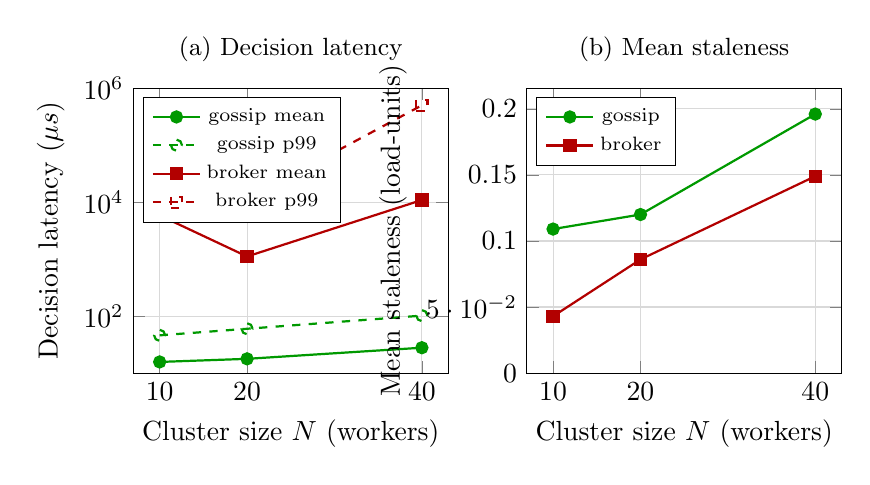
\begin{tikzpicture}
\begin{semilogyaxis}[
  width=0.46\textwidth, height=5.2cm,
  xlabel={Cluster size $N$ (workers)},
  ylabel={Decision latency ($\mu s$)},
  xtick={10,20,40},
  legend pos=north west,
  legend style={font=\scriptsize},
  ymin=10, ymax=1e6,
  grid=both, major grid style={gray!30}, minor grid style={gray!10},
  title={(a) Decision latency},
  title style={font=\small},
  name=plota,
]
\addplot[mark=*, thick, green!60!black] coordinates { (10,15.7) (20,17.8) (40,27.9) };
\addlegendentry{gossip mean};
\addplot[mark=o, thick, green!60!black, dashed] coordinates { (10,46) (20,60) (40,102) };
\addlegendentry{gossip p99};
\addplot[mark=square*, thick, red!70!black] coordinates { (10,5857.7) (20,1113.1) (40,10896.4) };
\addlegendentry{broker mean};
\addplot[mark=square, thick, red!70!black, dashed] coordinates { (10,501328) (20,11218) (40,500831) };
\addlegendentry{broker p99};
\end{semilogyaxis}
\begin{axis}[
  at={(plota.east)}, anchor=west, xshift=1cm,
  width=0.46\textwidth, height=5.2cm,
  xlabel={Cluster size $N$ (workers)},
  ylabel={Mean staleness (load-units)},
  xtick={10,20,40},
  legend pos=north west,
  legend style={font=\scriptsize},
  ymin=0,
  grid=both, major grid style={gray!30}, minor grid style={gray!10},
  title={(b) Mean staleness},
  title style={font=\small},
]
\addplot[mark=*, thick, green!60!black] coordinates { (10,0.109) (20,0.12) (40,0.196) };
\addlegendentry{gossip};
\addplot[mark=square*, thick, red!70!black] coordinates { (10,0.043) (20,0.086) (40,0.149) };
\addlegendentry{broker};
\end{axis}
\end{tikzpicture}
\caption{Decision latency (log scale, panel a) and routing-decision staleness
(panel b) for the locally-resolved gossip mode and the broker-mediated mode
on the same Mycelium substrate. Each point is the aggregate of one 20-second
run at 50 decisions/second. Gossip mean grows from 15.7 to 27.9 $\mu s$ over a
4$\times$ cluster scale; broker mean is two to three orders of magnitude
higher and p99 includes timeouts at the RPC ceiling.}
\label{fig:coordinator-latency}
\end{figure}


Table~\ref{tab:empirical} reports the aggregate per-run metrics; the same
data appears as Figure~\ref{fig:coordinator-latency}.

\begin{table}[t]
\centering
\small
\begin{tabular}{lrrrrr}
\toprule
\textbf{Mode} & \textbf{$N$} & \textbf{Mean ($\mu s$)} & \textbf{p95 ($\mu s$)} & \textbf{p99 ($\mu s$)} & \textbf{Mean staleness} \\
\midrule
gossip & 10 &     15.7 &    28 &     46 & 0.109 \\
broker & 10 &  5\,857.7 & 1\,428 & 501\,328 & 0.043 \\
gossip & 20 &     17.8 &    38 &     60 & 0.120 \\
broker & 20 &  1\,113.1 & 6\,933 &  11\,218 & 0.086 \\
gossip & 40 &     27.9 &    61 &    102 & 0.196 \\
broker & 40 & 10\,896.4 & 27\,912 & 500\,831 & 0.149 \\
\bottomrule
\end{tabular}
\caption{Aggregate metrics from a single $20$-second run per $(mode, N)$ pair
at $50$\,Hz decision rate. Staleness is the absolute difference between
\emph{perceived\_load} (used by the decision) and \emph{true\_load}
(measured at action time). The broker p99 values at $N{=}10$ and $N{=}40$
include decisions that hit the $500$\,ms RPC timeout entirely.}
\label{tab:empirical}
\end{table}

\textbf{Decision latency.} Gossip mode mean latency grows from $15.7$ to
$27.9$\,$\mu s$ across a $4\times$ cluster scale. This is consistent with
the framework's prediction: a locally-resolved decision is a scan of the
client's local KV, with cost linear in the number of entries scanned, and
that cost stays in the tens of microseconds at the tested scale. Broker
mode mean latency is between $1$\,ms and $11$\,ms — two to three orders
of magnitude higher than gossip — and the p99 tail includes the $500$\,ms
RPC timeout at $N{=}10$ and $N{=}40$. The substrate is not slow; the
serialisation through a single coordinating agent is. This is the
quantitative expression of the Coordinator Trap in one HLKS instantiation.

\textbf{Staleness.} The mean per-decision staleness — the magnitude by which
the perceived load differs from the actual load — is small in both modes
but consistently larger in broker mode at $N{=}40$ than the gossip mean
at any tested $N$. The broker's view is one gossip-round stale plus the
RPC round-trip; the client's local view is one gossip-round stale only.
The broker's lower staleness at $N{=}10$ reflects an artefact of the
small-cluster regime where the broker's gossip view converges quickly and
the broker's reduced effective decision rate (it answers fewer requests
per second) means each one is, on average, sampled closer to a load update.
The pattern reverses at $N{=}20$ and $N{=}40$, with broker staleness
exceeding gossip staleness at the largest tested cluster.

\textbf{Throughput.} Gossip mode achieved $743$--$901$ completed decisions
per $20$-second window; broker mode achieved $499$--$724$. The substrate
itself is not the constraint — the throughput gap is the broker's
serialisation behaviour at the tested decision rate.

\subsection{What the Measurement Establishes}

The broker-vs-gossip measurement establishes that, within the prediction
paradigm, moving the predictor from the centre to the edge yields the
latency and staleness improvements that Theorem~\ref{thm:coordtrap}
predicts as $\lambda$ shrinks---the gap is measurable in microseconds and
in tail latency that includes hard timeouts. It also establishes the
architectural-flexibility claim: the patterns are configurations of the
same substrate, compared with all confounders held constant. It does
\emph{not} establish a scaling law (three single-run data points do not
characterise asymptotics), and---per the framing above---it does not and
cannot validate the pull claim, which the next subsection addresses by
construction.

\subsection{The Pull Instantiation: \texttt{mycelium-tuple-space}}
\label{sec:pullinstantiation}

The pull grade of \S\ref{sec:twogrades} is realised as a companion crate
implementing generative communication in the lineage of
Linda~\cite{gelernter1985}: producers \texttt{put} work items into a named
stage; workers block on \texttt{take} and receive an item exactly when
they are ready; a worker advances a pipeline atomically with
\texttt{complete} (acknowledge the consumed item AND emit its successor in
one write-ahead-log record, so no crash window exists between stages).
Linda's classical weakness---the shared space as a designed-in
coordinator requiring its own consistency machinery---is addressed by
building the space's availability out of the substrate's own emergent
mechanisms, and its decision authority out of existence:

\begin{itemize}
\item \textbf{The space decides nothing.} It holds no model of any
  worker's state, makes no allocation decision, and predicts nothing.
  Allocation \emph{is} the workers' pull operations. The space is a
  rendezvous point on the data path---a capacity concern, like any shared
  medium---not an epistemic authority. The Coordinator Trap is a theorem
  about the latter; conflating the two is a category mistake the
  measurement vocabulary makes visible: no quantity in the system
  corresponds to ``misroute.''
\item \textbf{Failure handling is the substrate's, not a protocol's.} The
  serving node advertises a capability with the standard evaporation
  convention; a standby mirrors items via replication and promotes itself
  when the advertisement evaporates---failure detection \emph{is} the
  capability ring. Role election under the \texttt{Auto} policy is
  likewise emergent (candidates observe the ring and self-assign, with a
  deterministic lowest-identifier tie-break), matching the
  designed-in-versus-emergent distinction of \S\ref{sec:emergent}: the
  failover coalition forms from local rules in response to a specific
  event and holds no standing authority over the substrate.
\item \textbf{Promise minimalism, mechanically enforced.} The one residual
  future-promise (\S\ref{sec:promisereading})---a claiming worker's
  ``complete or release''---is not trusted: claims carry a deadline, and
  an expired claim returns the item to availability (at-least-once
  delivery). Saturation is announced by the stigmergic convention the
  substrate already uses---a pressure entry with read-side freshness that
  producers consult before spending a request---rather than by a
  flow-control protocol.
\end{itemize}

The behavioural claims are verified by the crate's test suite against real
clusters (loopback TCP and a five-node Docker deployment; all counts at
the commit accompanying this paper). Three results carry the empirical
weight:

\begin{enumerate}
\item \textbf{Exactness without prediction.} Ten concurrent producers and
  ten concurrent workers exchange 1{,}000 items with exactly-once
  delivery, and a parked worker receives a direct hand-off when work
  arrives---demonstrating that allocation precision under pull comes from
  the claim operation itself, with no participant ever holding a view of
  another's load.
\item \textbf{Survival of the rendezvous point.} With a primary and a
  mirroring standby, the primary is killed while three unacknowledged
  items are live: the standby detects the evaporation, promotes, and
  serves the three items under their \emph{original} identifiers;
  acknowledged items do not resurrect; identifier allocation is fenced
  past the dead primary's. The data-path availability concern is thereby
  shown to be solved by the same emergent mechanisms as everything else
  on the substrate---no external consistency service, the historical
  objection to tuple spaces.
\item \textbf{End-to-end pull across nodes.} The full integration scenario
  drives put/take/complete/acknowledge across distinct cluster nodes
  through the substrate's HTTP gateway, including in-flight accounting
  and the blocking-take timeout contract---the worker-loop shape that
  language SDKs (Python, TypeScript) expose to applications.
\end{enumerate}

\subsection{What Remains Open Empirically}

The definitive comparison this section sets up but does not yet report is
the three-arm experiment on one substrate: prediction-central (broker),
prediction-local (gossip), and pull (tuple space), under heterogeneous and
drifting service-time distributions. Because pull abolishes the
staleness/misroute vocabulary, the common metrics must be outcome-level:
end-to-end job latency distribution, throughput, idle-while-work-exists
time, and fairness under worker heterogeneity $H$. The framework's
prediction is specific: the gap between the prediction arms and the pull
arm widens monotonically with $H$ and with the state-change rate
$\bar{\delta}$, and the homogenisation corollary
(\S\ref{sec:homogenisation}) predicts the prediction arms recover
\emph{only} as workers are made clone-like. The binaries, the crate, and
the figure pipeline for this experiment are in the repository.

The results also do not transfer automatically to the other three domains.
The HLKS framework predicts that the same qualitative gap should appear in
appropriately analogous comparisons in market economies, governance
institutions, and organisational structures---Hayek's calculation problem,
Ostrom's commons-governance comparisons, and Beinhocker's corporate
performance data each provide existing empirical grounds in their
domain---but the present evidence establishes it directly only in
computing. Cross-domain empirical consilience is open work.

% ─────────────────────────────────────────────────────────────────────────────
\section{Open Questions}
\label{sec:open}

The argument as stated has boundary conditions and open questions that an
honest treatment must acknowledge. We list five.

\subsection{The Formal Status of the Coordinator Trap Theorem}

We have argued in \S\ref{sec:formalstatus} that the cross-domain claim is
correctly stated informally and that domain-specific formal proofs exist for
specific instantiations. A complete treatment would either: (a)~prove the
theorem formally in a parametric model that admits the four domain
specialisations as instances, or (b)~argue carefully that no such parametric
model can capture all four without losing the cross-domain generality, in
which case the informal statement is the strongest available form. We
incline toward (b), but a defensible argument for either position would
substantially clarify the foundations.

\subsection{HLKS Boundary Conditions}

The Coordinator Trap Theorem depends on heterogeneity (condition (i)) and
non-zero state-change rates (condition (ii)). There exist systems in which
these conditions fail: a database with identical replicas and infrequent
writes is better served by traditional consensus than by gossip; a
homogeneous worker pool with bounded turnover may not benefit from local
resolution. The framework's claim is scoped to HLKS systems; it must state
explicitly where the boundary lies and what evidence would establish whether
a given system is inside or outside it. The literature on the homogeneous
versus heterogeneous distinction in distributed systems is rich but
unsettled; an HLKS-specific characterisation is open work.

\subsection{Quantitative Operationalisation of MCB/P/S}

As stated, MCB, P, and S are qualitative axes. The original monetary system
literature treats them as evaluative dimensions rather than precise metrics.
A complete cross-domain framework should investigate whether any of the three
can be quantified in a way that is consistent across domains, enabling, for
example, a numeric comparison of the polycentricity of monetary versus
computing versus governance substrates on the same scale. We suspect P admits
quantification (the fraction of decisions made locally is observable in
principle); MCB and S are more difficult.

\subsection{The Holland/Burgess Reading of Property 4}

\S\ref{sec:emergent} argues that Holland's CAS framework and Burgess's
Promise Theory are not in genuine tension on emergent consensus---both can
accommodate it under a careful reading. A complete treatment should engage
directly with Burgess's response. He would likely argue that the framework's
emergent consensus is a legitimate Promise-Theory structure, but might
question whether the substrate-level claim (consensus is justified for the
specific class of operations requiring binding cross-agent commitment) is
sharp enough to prevent re-importation of a coordinator under the
``emergent'' label. The diagnostic test in \S\ref{sec:properties}---``can
this operation tolerate eventual consistency?''---is intended to be that
sharp criterion, but its empirical application across domains is open work.

\subsection{Properties Beyond Epistemic Correctness}

A substrate satisfying Properties 1--4 is epistemically correct: it solves
the coordinator-trap problem the framework identifies. It is not, however,
necessarily resistant to political capture. Two further failure modes are
visible empirically and require structural treatment that the present paper
does not provide:
\begin{itemize}
\item \emph{External capture}: a substrate satisfying Properties 1--4 may
  still be captured by concentrated external interests who acquire control of
  the emergent consensus mechanisms (Property 4) and bend them to extract
  coordination rent. The cost of capture and the rents it yields are not
  symmetric; the asymmetry is the subject of Olson's analysis of collective
  action and bears directly on substrate design.
\item \emph{Internal capture}: a substrate satisfying Properties 1--4, and
  hardened against external capture, may still be captured from within by the
  agents who operate the consensus mechanisms. Standing tenure in a
  coordination role accumulates informational, relational, and normative
  advantages that compound over time, producing a structurally permanent
  coordination class even when formal authority rotates.
\end{itemize}
A companion paper currently in preparation introduces three further
properties---Capture Resistance, Mandate TTL, and Epistemic Symmetry---that
address these failure modes, and develops the corresponding empirical
analysis in monetary, political, and computing contexts. The present paper
limits its scope to the four properties that follow directly from the
Coordinator Trap Theorem; the further three follow from political-economic
considerations that the theorem does not entail.

% ─────────────────────────────────────────────────────────────────────────────
\section{Conclusion}

The central claim of this paper, restated precisely: we are not arguing that
all complex systems should be coordinator-free, or that consensus is never
appropriate. We are arguing that for any system satisfying the HLKS
conditions---heterogeneous agents, local knowledge, non-zero state-change
rates---a coordinator-based substrate accumulates epistemic error
proportional to scale, heterogeneity, and the rate of state change, while a
locally-resolved signal substrate with minimal federation invariants and
subsidiarity-respecting consensus does not. The four traditions
(Hayek, Ostrom, Beinhocker, and the Holland/Nicholson computing line)
converge on Properties 1--4 because they are independently solving the same
HLKS problem in four different domain vocabularies. The convergence is the
evidence; the HLKS framework is the explanation.

The companion paper~\cite{nicholson2026} characterised the convergence as
``suggestive rather than exact.'' That qualification was honest given the
single-domain scope of that paper. With the HLKS framework, the qualification
can be removed: the parallel is exact, because the four domains are
instantiations of the same formal problem. The structural identity of
Table~\ref{tab:identity} is the precise statement of what ``exact'' means
here: each component of the HLKS framework has a specific form in each
domain, and the substrate properties follow from the framework in each
domain identically.

For substrate architects, the practical implication is direct. Before
designing a substrate for any domain with heterogeneous agents and local
knowledge, the architect should: identify the HLKS components in the target
domain; compute or estimate the coordinator's epistemic error at the target
scale; design for local resolution wherever the operation admits it;
minimise the federation invariants; apply the subsidiarity test before
invoking consensus; and evaluate the resulting substrate on the MCB/P/S
axes. The same set of design moves applies whether the substrate is a
monetary system, a governance institution, an organisational structure, or
a distributed computing platform.

For HLKS theory, the practical implication is that the cross-domain
framework opens specific lines of further work: formal proof in a parametric
model, quantitative operationalisation of MCB/P/S, empirical
characterisation of HLKS boundary conditions, and---most importantly---the
political-economy properties (external and internal capture resistance) that
the present paper deliberately leaves to its companion. The four traditions
converged on the same epistemic answer because the problem is the same. They
have not yet converged on the political-economy answer; the companion paper
argues that they should.

\section*{Acknowledgements}

This paper grew out of an extended development of the ideas in the companion
paper~\cite{nicholson2026}. The author thanks the contributors to the
Mycelium project for sustained engagement with the substrate-level claims,
and the readers who pushed back on the original ``suggestive rather than
exact'' qualification with the observation that the parallel might be made
exact with the right abstraction. That observation is the seed of the
present paper.

% ─────────────────────────────────────────────────────────────────────────────
\bibliography{references}

\end{document}
